%%%%%%%%%%%%%%%%%%%%%%%%%%%%%%%%%
% Writing Game Theory in LaTeX
% Original author:
% Thiago Nascimento da Silva
%%%%%%%%%%%%%%%%%%%%%%%%%%%%%%%%%

%----------------------------------------------------------------------------------------
%	PACKAGES AND OTHER DOCUMENT CONFIGURATIONS
%----------------------------------------------------------------------------------------

\documentclass[12pt]{article} % Page size
\usepackage[utf8]{inputenc} % Input encoding and font encoding 
\usepackage[margin = 1in]{geometry} % Margins  
\usepackage{setspace} % Setting the spacing between lines
\usepackage{amsthm, amsmath, amsfonts, mathtools, amssymb} % Math packages 
\usepackage{sgame, tikz} % Game theory packages
\usetikzlibrary{trees, calc} % For extensive form games
\usepackage{subfig} % Manipulation and reference of small or sub figures and tables
\usepackage{hyperref} % To create hyperlinks within the document
\hypersetup{
    colorlinks=true, % true if you want colored links
    linktoc=all,     % set to all if you want both sections, subsections, and numbers linked
    linkcolor=blue,  %choose some color if you want links to stand out
}

\def\table{\def\figurename{Table}\figure} % necessary to merge the list of tables with the list of figures
\let\endtable\endfigure % necessary to merge the list of tables with the list of figures



%============Article Title, Author================
\title{Writing Game Theory in \LaTeX}
\author{Thiago Silva\thanks{PhD Candidate, Department of Political Science, Texas A\&M University, College Station, TX, 77843-4348, USA. E-mail: nsthiago@tamu.edu}}
\date{First Version: November 22, 2015\\
This Version: \today
}

%===================Startup========================
\begin{document} 
\maketitle

\thispagestyle{empty} % removing page number for the first page

\renewcommand\listfigurename{\large{List of Figures and Tables}} % Giving the name List of Figures and Tables to \listoffigures
\listoffigures



\clearpage

\doublespace

%%%%%%%%%%%%%%%%%%%%%%%%%%%%%%%%%%%%%%%%%%%%%%
%
% GAME THEORY
%
%%%%%%%%%%%%%%%%%%%%%%%%%%%%%%%%%%%%%%%%%%%%%%

In order to present how to write game theory in \LaTeX, I will use the most popular game in game theory called the Prisoner's Dilemma (PD) as an example. The PD shows why two rational individuals might not cooperate even if cooperation is in their best interest, thus resulting in a sub-optimal outcome. The game was formalized and named by Albert Tucker.\footnote{See Poundstone, William. 1992 \emph{Prisoner's Dilemma}. New York City: Anchor Books.}


%%%%%%%%%%%%%%%%%%%%%%%%%%%%%%%%%%%%%%%%%%%%%%
%
% Prisoner's Dilemma in static or normal-form
%
%%%%%%%%%%%%%%%%%%%%%%%%%%%%%%%%%%%%%%%%%%%%%%


The Prisoner's Dilemma (in static or normal-form game) consist of:
\begin{itemize}
	\item \textbf{A set of players} $N$, and $N = \{1, 2\}$, where $1$ stands for ``Player 1'' and $2$ stands for ``Player 2.''
	\item For each $i \in N$, a set of actions $S_{i}$---that is, \textbf{a set of actions} or {a set of strategies}---$S_{i} = \{C, D\}$, where $C$ stands for ``Cooperate'' and $D$ stands for ``Defect.'' In PD $S_{1} = S_{2} = \{C,D\}$.
	\item For each $i \in N$, a \textbf{preference relation} $\succsim_{i}$ over $S_{1} \times S_{2}$ (i.e., the Cartesian product). Instead of outcome, we usually use the term \emph{action profiles} (or strategy profiles), i.e., a combination of actions such as (DC), (CC), and so on. Players care about their actions, because their actions lead to action profiles that have payoff utilities assigned to them. Each player has a utility function $v_{i}:S_{1}\times S_{2} \rightarrow \mathbb{R}$. For any collection of sets $S_{1}, S_{2}, \dots, S_{n}$, we define $S_{1} \times S_{2} \times \dots \times S_{n} = \{(s_{1}, s_{2}, \dots, s_{n})|s_{1}\in S_{1}, \dots, s_{n}\in S_{n}\}$. We call $(s_{1}, s_{2}, \dots, s_{n})$ the ordered ``n-tuples'' ordered pairs $(s_{1}, s_{2})$. This is important to show that $(1,2) \neq (2,1)$. For PD game $S_{1}\times S_{2} = \{CC, CD, DC, DD\}$. 
	
	\end{itemize}
	
	The ordering of the action profiles, from best to worst---where the first action in parentheses represents player 1's action and the second action represents player 2's action---is $(D, C)$, where player $1$ defects and player $2$ cooperates; $(C, C)$, where both $1$ and $2$ cooperate; $(D, D)$, where both $1$ and $2$ defect, and; $(C, D)$, where $1$ cooperates and $2$ defects. 


The players' preferences can be represented according to payoff functions. First, we assign a utility function $u$, such as $u_{1}$ for player 1, and $u_{2}$ for player 2. We can express the order of players' preferences as, 
\begin{equation}
	\begin{array}{l} %{l} for left aligned array
		\text{For player $1$:}\\
		u_{1} (D, C) > u_{1} (C, C) > u_{1} (D, D) > u_{1} (C, D)\\
		\\
		\text{For player $2$:}\\
		u_{2} (C, D) > u_{2} (C, C) > u_{2} (D, D) > u_{1} (D, C)
		\end{array}
	\end{equation}
	
Then, we can assign the respective payoffs,
\begin{equation}
	\begin{array}{l}
		\text{For $P_{1}$:}\\
		u_{1} (D, C) = 3 > u_{1} (C, C) = 2 > u_{1} (D, D) = 1 > u_{1} (C, D) = 0\\
		\\
		\text{For $P_{2}$:}\\
		u_{2} (C, D) = 3 > u_{2} (C, C) = 2 > u_{2} (D, D) = 1 > u_{2} (D, C) = 0\\
		\end{array}
	\end{equation}

We can represent the game in a payoff matrix, also called ``normal-form game'':

\vskip.20in % vertical space between the last paragraph and the figure 
	
%%%%%%%%%%%%%%%%%%%%%%%%%%%%%%%%%%%%%%%%%%%%%%
%
% 2x2 Matrix: Prisoner's Dilemma
%
%%%%%%%%%%%%%%%%%%%%%%%%%%%%%%%%%%%%%%%%%%%%%%	
	
\begin{table}[!htbp] % Each letter of htbp stands for h=here; t=top; b=bottom; p=page of float
\centering
	\caption{2x2 Matrix: Prisoner's Dilemma Normal-Form Game \label{prisoners}}  %The use of the star * after caption is to remove the text "Table" from the title
\begin{game}{2}{2}[Player 1][Player 2]
	    &  C      &  D     \\
	 C  &  $2, 2$ & $0, 3$  \\
	 D  &  $3, 0$ & $1, 1$\\
\end{game}
\end{table}

The traditional Prisoners's Dilemma can be generalized from its original setting (see the right matrix below): If both players cooperate, they both receive the reward payoff $R$ for cooperating. If both players defect, they both receive the punishment payoff $P$. If $1$ defects while $2$ cooperates, then $1$ receives the temptation payoff $T$, while $2$ receives the ``sucker's'' payoff, $S$. Symmetrically, if $1$ cooperates while $2$ defects, then $1$ receives the sucker's payoff $S$, while $2$ receives the temptation payoff $T$.

\vskip.20in % vertical space between the last paragraph and the figure


%%%%%%%%%%%%%%%%%%%%%%%%%%%%%%%%%%%%%%%%%%%%%%%%%%%%%%%
%
% Two Matrices: Generalization of Prisoner's Dilemma
%
%%%%%%%%%%%%%%%%%%%%%%%%%%%%%%%%%%%%%%%%%%%%%%%%%%%%%%%



\begin{figure}[htbp]
	\centering
	\caption{Two Matrices: Generalization of Prisoner's Dilemma}\label{twomatrices}
\begin{minipage}{.5\textwidth}
   \begin{game}{2}{2}[$P_{1}$][$P_{2}$]
   	    &  Cooperate     &  Defect     \\
   	 Cooperate  &    $2, 2$      & $0, 3$  \\
   	 Defect &  $3, 0$ & $1, 1$\\
   \end{game}
\end{minipage}% This must go next to `\end{minipage}`
\begin{minipage}{.5\textwidth}
   \begin{game}{2}{2}[$P_{1}$][$P_{2}$]
   	    &  Cooperate      &  Defect     \\
   	 Cooperate  &    $R, R$      & $S, T$  \\
   	 Defect &  $T, S$ & $P, P$\\
   \end{game}
\end{minipage}
\end{figure}

\vskip.20in % vertical space between the figure and the next paragraph

Finding the Nash equilibrium (NE) of the Prisoner's Dilemma (PD) game: The action profile $a^{*}$ in a strategic game with ordinal preferences is a Nash equilibrium if, for every player $i$ and every action $a_{i}$ of player $i$, $a^{*}$ is at least as good according to player $i$'s preferences as the action profile $(a_{i}, a^{*}_{-i})$ in which player $i$ chooses $a_{i}$ while every other player ${-i}$, with $i \neq -i$, chooses $a^{*}_{-i}$. Therefore, for every player $i$
\begin{equation}
u_{i}(a^{*}) \geq u_{i}(a_{i}, a^{*}_{-i}) \, \forall \, a_{i} \in A_{i}
\end{equation}
where $A_{i}$ is the set of actions for player $i$, and $u_{i}$ is a payoff function that represents player $i$'s preferences.


%%%%%%%%%%%%%%%%%%%%%%%%%%%%%%%%%%%%%%%%%%%%%%%%%%%%%%%%%%%%%%%%%%%%%%%%%%%%%%%%%%%%%%%%%%%
%
% Finding the Nash Equilibrium of Prisoner's Dilemma underlining players' best responses
%
%%%%%%%%%%%%%%%%%%%%%%%%%%%%%%%%%%%%%%%%%%%%%%%%%%%%%%%%%%%%%%%%%%%%%%%%%%%%%%%%%%%%%%%%%%%

\begin{table}[htbp]
\centering
	\caption{Finding the Nash Equilibrium of Prisoner's Dilemma (Underlining Players' Best Responses) \label{NEprisoners}}  
\begin{game}{2}{2}[Player 1][Player 2]
	    &  C       &  D    \\
	 C  &  $2, 2$  & $0, \underline{3}$  \\
	 D  &  $\underline{3}, 0$ & $\underline{1}, \underline{1}$\\
\end{game}
\end{table}

Each underlined action indicates the best response of each player according to the other player's action. Therefore, $NE = (D, D)$.

The PD can also be depicted in a game of extensive-form (or decision tree), such as:


\vskip.30in % vertical space between the figure and the next paragraph

%%%%%%%%%%%%%%%%%%%%%%%%%%%%%%%%%%%%%%%%%%%
%
% Prisoner's Dilemma in Extensive-form
%
%%%%%%%%%%%%%%%%%%%%%%%%%%%%%%%%%%%%%%%%%%%

 \begin{figure}[htbp]
 	\centering
	\caption{Prisoner's Dilemma in Extensive-form \label{PDExtensive}}
    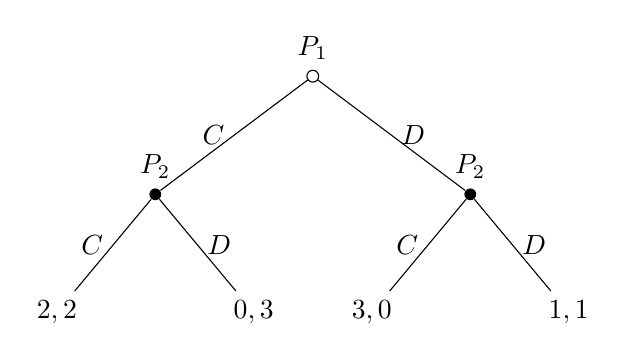
\begin{tikzpicture}[thin,
      level 1/.style={sibling distance=40mm},
      level 2/.style={sibling distance=25mm},
      level 3/.style={sibling distance=15mm},
      every circle node/.style={minimum size=1.5mm,inner sep=0mm}]
      
      \node[circle,draw,label=above:$P_{1}$] (root) {}
        child { node [circle,fill,label=above:$P_{2}$] {}
          child { 
            node {$2,2$}
            edge from parent
              node[left] {$C$}}
          child { 
            node {$0,3$}
            edge from parent
              node[right] {$D$}}
          edge from parent
            node[left] {$C$}}
        child { node [circle,fill,label=above:$P_{2}$] {}
          child { 
            node {$3,0$}
              edge from parent
                node[left] {$C$}}
          child { 
            node {$1,1$}
              edge from parent
                node[right] {$D$}}
           edge from parent
             node[right] {$D$}};
    \end{tikzpicture}
  \end{figure}
  
  
  \vskip.30in % vertical space between the figures

%%%%%%%%%%%%%%%%%%%%%%%%%%%%%%%%%%%%%%%%%%%%%%%%%%%%%%%%%%%%%%%%%%%%%%%%%%%%%%%%%%%%%%%%%%%%%%%%%%%%%%%%
%
% Finding the Subgame Perfect Nash Equilibrium in Prisoner's Dilemma using Double Lines
%
%%%%%%%%%%%%%%%%%%%%%%%%%%%%%%%%%%%%%%%%%%%%%%%%%%%%%%%%%%%%%%%%%%%%%%%%%%%%%%%%%%%%%%%%%%%%%%%%%%%%%%%%

 \begin{figure}[htbp]
 	\centering
	\caption{Finding the Subgame Perfect Nash Equilibrium in Prisoner's Dilemma (Using Double Lines) \label{PDSPE}}
    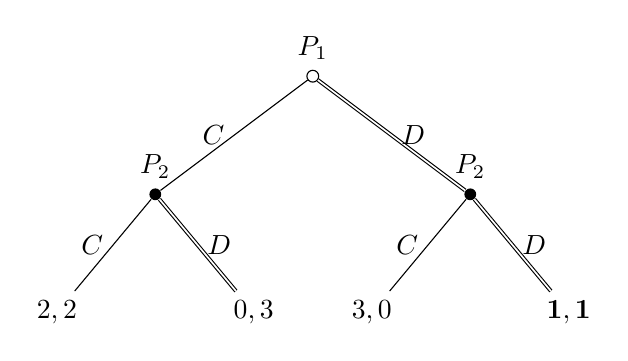
\begin{tikzpicture}[thin,
      level 1/.style={sibling distance=40mm},
      level 2/.style={sibling distance=25mm},
      level 3/.style={sibling distance=15mm},
      every circle node/.style={minimum size=1.5mm,inner sep=0mm}]
      
      \node[circle,draw,label=above:$P_{1}$] (root) {}
        child { node [circle,fill,label=above:$P_{2}$] {}
          child { 
            node {$2,2$}
            edge from parent
              node[left] {$C$}}
          child { 
            node {$0,3$}[double] % [double] specifies the double line
            edge from parent
              node[right] {$D$}}
          edge from parent
            node[left] {$C$}}
        child { node [circle,fill,label=above:$P_{2}$] {}
          child { 
            node {$3,0$}
              edge from parent
                node[left] {$C$}}
          child { 
            node {$\mathbf{1,1}$}
              edge from parent
                node[right] {$D$}[double]}
           edge from parent
             node[right] {$D$}[double]};
    \end{tikzpicture}
  \end{figure}

\clearpage
%%%%%%%%%%%%%%%%%%%%%%%%%%%%%%%%%%%%%%%%%%%%%%%%%%%%%%%%%%%%%%%%%%%%%%%%%%%%%%%%%%%%%%%%%%%%%%%%%%%%%%%%

\section*{Other Examples and Game Forms}

%%%%%%%%%%%%%%%%%%%%%%%%%%%%%%%%%%%%%%%%%%%%%%%%%%%%%%%%%%%%%%%%%%%%%%%%%%%%%%%%%%%%%%%%%%%%%%%%%%%%%%%%


%%%%%%%%%%%%%%%%%%%%%%%%%%%%%%%%%%%%%%%%%%%%%%%%
%
% Finding the Nash Equilibrium using dots
%
%%%%%%%%%%%%%%%%%%%%%%%%%%%%%%%%%%%%%%%%%%%%%%%%

\begin{table}[!htbp]
\centering
	\caption{Finding the Nash Equilibrium (Using Dots) \label{dots}}  
\begin{game}{2}{2}[Player 1][Player 2]
	    &  C       &  D    \\
	 C  &  $2, 2$  & $0,\dot{3}$  \\
	 D  &  $\dot{3}, 0$ & $\dot{1}, \dot{1}$\\
\end{game}
\end{table}

%%%%%%%%%%%%%%%%%%%%%%%%%%%%%%%%%%%%%%%%%%%%%%%%

The small dot on top of each payoff indicates the best response of each player according to the other player's action. \textbf{Note:} Be careful to not confuse strategy profiles (or outputs) with payoff utilities (i.e., $(D,D)\neq(1,1)$). The equilibrium (or equilibria) of a game refers to the strategy profile(s). Therefore, $NE = (D, D)$.

%%%%%%%%%%%%%%%%%%%%%%%%%%%%%%%%%%%%%%%%%%%%%%%%%%%%%%%%%%%%%%%%%%%%%%%%%%%%%%%%%%%%%%%%%%%%%%%%%
%
% An alternative depiction of players' strategy profiles and their respective payoff utilities
%
%%%%%%%%%%%%%%%%%%%%%%%%%%%%%%%%%%%%%%%%%%%%%%%%%%%%%%%%%%%%%%%%%%%%%%%%%%%%%%%%%%%%%%%%%%%%%%%%%


\vskip.40in % vertical space between examples


		   
%%%%%%%%%%%%%%%%%%%%%%%%%%%%%%%%%%%%%%%%%%%%%%%%
%
% 3x3 Matrix: A game with three actions
%
%%%%%%%%%%%%%%%%%%%%%%%%%%%%%%%%%%%%%%%%%%%%%%%%

\begin{table}[!htbp]
\centering
	\caption{3x3 Matrix: A Game with Three Actions \label{threeactions}}  
\begin{game}{3}{3}[Player 1][Player 2]
   	    &  Cooperate                 &  Defect  & Neither   \\
   	 Cooperate  &    $R, R$      & $S, T$ & $T, S$ \\
   	 Defect &  $T, S$ & $P, P$ & $R, S$\\
	 Neither &  $T, S$ & $P, P$ & $S, S$\\
\end{game}
\end{table}

\vspace{2em}

%%%%%%%%%%%%%%%%%%%%%%%%%%%%%%%%%%%%%%%%%%%%%%%%%%%%%%%%%%%%%%%%%%%%%%%%%%%%%%%%%%%%%%%%%%%%%%%%%%%%%%%%
%
% 2x4 Matrix: A game with 2 actions for Player 1  and 4 actions for Player 2
%
%%%%%%%%%%%%%%%%%%%%%%%%%%%%%%%%%%%%%%%%%%%%%%%%%%%%%%%%%%%%%%%%%%%%%%%%%%%%%%%%%%%%%%%%%%%%%%%%%%%%%%%%

\begin{table}[!htbp]
\centering
	\caption{2x4 Matrix: A Game with Two Actions for $P_{1}$ and Four Actions for $P_{2}$ \label{twobyfour}}  
\begin{game}{2}{4}[$P_{1}$][$P_{2}$]
   	&   C Unconditionally &  D Unconditionally & Imitation Move  &  Opposite Move   \\
   	 C  &    $R, R$      & $S, T$ & $R, R$ & $S, T$\\
   	 D &  $T, S$ & $P, P$ & $P, P$ & $T, S$\\
\end{game}
\end{table}

%%%%%%%%%%%%%%%%%%%%%%%%%%%%%%%%%%%%%%%%%%%%%%%%%%%%%%%%%%%%%%%%%%%%%%%%%%%%%%%%%%%%%%%%%%%%%%%%%%%%%%%%
%
% Bach or Stravinsky (Battle of the sexes game)
%
%%%%%%%%%%%%%%%%%%%%%%%%%%%%%%%%%%%%%%%%%%%%%%%%%%%%%%%%%%%%%%%%%%%%%%%%%%%%%%%%%%%%%%%%%%%%%%%%%%%%%%%%

\begin{table}[!htbp] % Each letter of htbp stands for h=here; t=top; b=bottom; p=page of float
\centering
	\caption{Bach or Stravinsky? \label{bos}}  %The use of the star * after caption is to remove the text "Table" from the title
\begin{game}{2}{2}[Player 1][Player 2]
	  	  		 &  Bach      &  Stravinsky     \\
	 Bach  		 &  $3, 2$ & $0, 0$  \\
	 Stravinsky  &  $0, 0$ & $2, 3$\\
\end{game}
\end{table}

%%%%%%%%%%%%%%%%%%%%%%%%%%%%%%%%%%%%%%%%%%%%%%%%%%%%%%%%%%%%%%%%%%%%%%%%%%%%%%%%%%%%%%%%%%%%%%%%%%%%%%%%
%
% The game of chicken (the hawk-dove game)
%
%%%%%%%%%%%%%%%%%%%%%%%%%%%%%%%%%%%%%%%%%%%%%%%%%%%%%%%%%%%%%%%%%%%%%%%%%%%%%%%%%%%%%%%%%%%%%%%%%%%%%%%%

\begin{figure}[htbp]
	\centering
	\caption{The Game of Chicken (The Hawk-Dove Game)}\label{chicken}
\begin{minipage}{.5\textwidth}
   \begin{game}{2}{2}[$P_{1}$][$P_{2}$]
   	    &  Swerve    &  Straight     \\
   	 Swerve  &    $0, 0$      & $-1, 1$  \\
   	 Straight &  $1, -1$ & $-10, -10$\\
   \end{game}
\end{minipage}% This must go next to `\end{minipage}`
\begin{minipage}{.5\textwidth}
   \begin{game}{2}{2}[$P_{1}$][$P_{2}$]
   	    &  Swerve    &  Straight     \\
   	 Swerve  &   Tie, Tie      & Lose, Win \\
   	 Straight &  Win, Lose & Crash, Crash\\
   \end{game}
\end{minipage}
\end{figure}

%%%%%%%%%%%%%%%%%%%%%%%%%%%%%%%%%%%%%%%%%%%%%%%%%%%%%%%%%%%%%%%%%%%%%%%%%%%%%%%%%%%%%%%%%%%%%%%%%%%%%%%%
%
% Matching pennies game
%
%%%%%%%%%%%%%%%%%%%%%%%%%%%%%%%%%%%%%%%%%%%%%%%%%%%%%%%%%%%%%%%%%%%%%%%%%%%%%%%%%%%%%%%%%%%%%%%%%%%%%%%%

\begin{table}[!htbp] 
\centering
	\caption{Matching Pennies \label{pennies}}  %The use of the star * after caption is to remove the text "Table" from the title
\begin{game}{2}{2}[Player 1][Player 2]
	  	  		 &  Heads      &  Tails     \\
	 Heads 		 &  $1, -1$ & $-1, 1$  \\
	 Tails       &  $-1, 1$ & $1, -1$\\
\end{game}
\end{table}



%%%%%%%%%%%%%%%%%%%%%%%%%%%%%%%%%%%%%%%%%%%%%%%%%%%
%
% Game with Mixed Strategies (Example 1)
%
%%%%%%%%%%%%%%%%%%%%%%%%%%%%%%%%%%%%%%%%%%%%%%%%%%%


\begin{table}[!htbp]
\centering
\caption{Game with Mixed Strategies (Example 1)\label{mix1}}  
\begin{game}{2}{2}[$P_{1}$][$P_{2}$]
			&   $(q)$   A  &  $(1-q)$ B \\
				$(p)$	A  &  $ \alpha, \beta $ & $ \epsilon, \zeta $  \\
				$(1-p)$	B  &  $ \gamma, \delta $ & $ \eta, \theta $ \\
			\end{game}
		\end{table}	
		
		
\clearpage %% Starting a new page

%%%%%%%%%%%%%%%%%%%%%%%%%%%%%%%%%%%%%%%%%%%%%%%%%%%
%
% Game with Mixed Strategies (Example 2)
%
%%%%%%%%%%%%%%%%%%%%%%%%%%%%%%%%%%%%%%%%%%%%%%%%%%%
		
	\begin{table}[!htbp]
		\centering
		\caption{Game with Mixed Strategies (Example 2)\label{mix2}}  
		\begin{game}{3}{2}[$P_{1}$][$P_{2}$]
			&   $ (q) $ D  &  $ (1 - q) $ E    \\
				$ (x) $	A  &  $ \iota, \kappa$ & $ o, \pi $  \\
				$ (y) $	B  &  $ \lambda, \mu$ & $ \rho,\sigma $ \\
				$ (1 - x - y) $	C  & $ \nu, \xi $ & $ \tau, \upsilon $ \\
		\end{game}
	\end{table}	

\vspace{2em}


%%%%%%%%%%%%%%%%%%%%%%%%%%%%%%%%%%%%%%%%%%%%%%%%%%%
%
% Centipede Game
%
%%%%%%%%%%%%%%%%%%%%%%%%%%%%%%%%%%%%%%%%%%%%%%%%%%%

\begin{figure}[!htbp]
\centering
\caption{Centipede Game\label{centipede}}
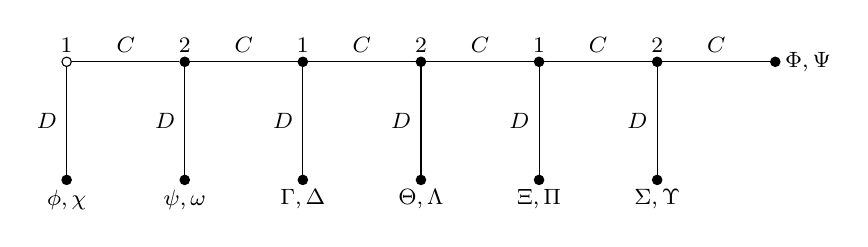
\begin{tikzpicture}[font=\footnotesize,scale=1]
% Two node styles: solid and hollow
\tikzstyle{solid node}=[circle,draw,inner sep=1.2,fill=black];
\tikzstyle{hollow node}=[circle,draw,inner sep=1.2];
% The Tree
\node(0)[hollow node]{}
child[grow=down]{node[solid node]{}
	edge from parent node[left]{$D$}}
child[grow=right]{node(1)[solid node]{}
child[grow=down]{node[solid node]{}
	edge from parent node[left]{$D$}}
child[grow=right]{node(2)[solid node]{}
child[grow=down]{node[solid node]{}
	edge from parent node[left]{$D$}}
child[grow=right]{node(3)[solid node]{}
child[grow=down]{node[solid node]{}
	edge from parent node[left]{$D$}}
child[grow=right]{node(4)[solid node]{}
child[grow=down]{node[solid node]{}
	edge from parent node[left]{$D$}}
child[grow=right]{node(5)[solid node]{}
child[grow=down]{node[solid node]{}
	edge from parent node[left]{$D$}}
child[grow=right]{node(6)[solid node]{}
edge from parent node[above]{$C$}}
edge from parent node[above]{$C$}}
edge from parent node[above]{$C$}}
edge from parent node[above]{$C$}}
edge from parent node[above]{$C$}}
edge from parent node[above]{$C$}};
	% Movers
\foreach \x in {0,2,4}
\node[above]at(\x){1};
\foreach \x in {1,3,5}
\node[above]at(\x){2};
	  % payoffs
\node[below]at(0-1){$\phi,\chi$};
\node[below]at(1-1){$\psi,\omega$};
\node[below]at(2-1){$\Gamma,\Delta$};
\node[below]at(3-1){$\Theta,\Lambda$};
\node[below]at(4-1){$\Xi,\Pi$};
\node[below]at(5-1){$\Sigma,\Upsilon$};
\node[right]at(6){$\Phi,\Psi$};
\end{tikzpicture}
\end{figure}


%%%%%%%%%%%%%%%%%%%%%%%%%%%%%%%%%%%%%%%%%%%%%%%%%%%%%%%%%%%%%%%%%%%%%%%%%%%%%%%%%%%%%%%%%%%%%
%
% Three Players Game: Combining Extensive Form and Matrix Form
%
%%%%%%%%%%%%%%%%%%%%%%%%%%%%%%%%%%%%%%%%%%%%%%%%%%%%%%%%%%%%%%%%%%%%%%%%%%%%%%%%%%%%%%%%%%%%%

	\begin{figure}[!htbp]
		\centering
		\caption{Three Players Game: Combining Extensive Form with Matrix Form}\label{hybrid1}
\begin{tikzpicture}
  \node(0)[circle,draw,inner sep=1.2,label=below:$P_3$]{}
    [grow'=north,sibling distance=5cm]
    child{edge from parent node[below left]{X}}
    child{edge from parent node[below right]{Y}}
  ;
  \node[anchor=south]at(0-1){
	    \begin{game}{2}{2}[$P_{1}$][$P_{2}$]
	           & X   & Y\\
	         X & $1, 1, 1$ & $2, 0, 2$\\
	         Y & $0, 2, 0$ & $2, 2, 2$
		   \end{game}
  };
  \node[anchor=south]at(0-2){
		   \begin{game}{2}{2}[$P_{1}$][$P_{2}$]
		        & X   & Y\\
		      X & $3, 1, 3$ & $2, 2, 2$\\
		      Y & $1, 1, 1$ & $1, 3, 1$
		     \end{game}
  };
\end{tikzpicture}
\end{figure}

%%%%%%%%%%%%%%%%%%%%%%%%%%%%%%%%%%%%%%%%%%%%%%%%%%%%%%%%%%%%%%%%%%%%%%%%%%%%%%%%%%%%%%%%%%%%%
%
% Alternative Three Players Game: Combining Extensive Form and Matrix Form
%
%%%%%%%%%%%%%%%%%%%%%%%%%%%%%%%%%%%%%%%%%%%%%%%%%%%%%%%%%%%%%%%%%%%%%%%%%%%%%%%%%%%%%%%%%%%%%
	   

\begin{figure}[!htbp]
	\centering
	\caption{Alternative Three Players Game: Combining Extensive Form with Matrix Form}\label{hybrid2}
	\begin{tikzpicture}[scale=1] % You can change the scale of your figure, e.g., scale=1.5 = 50% bigger
	  % Two node styles: solid and hollow
	    \tikzstyle{solid node}=[circle,draw,inner sep=1.2];
	    \tikzstyle{hollow node}=[circle,draw, inner sep=1.2];
	  % Specify spacing for each level of the tree
	    \tikzstyle{level 1}=[level distance=15mm,sibling distance=50mm]
	    \tikzstyle{level 2}=[level distance=15mm,sibling distance=25mm]
	  % The Tree
	  \node(0)[hollow node]{}
	    child{node{}
		edge from parent node[above left]{X}
	    }
	    child{node{}
		edge from parent node[above right]{Y}
	    };
	  % movers
	  \node[circle, label=above:{P3}]at(0){};
	  \node[below]at(0-1){
	    \arrayrulewidth.75pt
	    \begin{game}{2}{2}[$P_{1}$][$P_{2}$]
	           & X   & Y\\
	       X & $1, 1, 1$ & $2, 0, 2$\\
	       Y & $0, 2, 0$ & $2, 2, 2$
		   \end{game}
		     };
		     \node[below,xshift=-15]at(0-2){
		       \arrayrulewidth.75pt
		       \begin{game}{2}{2}[$P_{1}$][$P_{2}$]
		              & X   & Y\\
		          X & $3, 1, 3$ & $2, 2, 2$\\
		          Y & $1, 1, 1$ & $1, 3, 1$
		       \end{game}
		     };
		   \end{tikzpicture}
		   \end{figure}
		   

		 
\clearpage 



%%%%%%%%%%%%%%%%%%%%%%%%%%%%%%%%%%%%%%%%%%%%%%%%%%%%%%%%%%%%%%%%%%%%%%%%%%%%%%%%%%%%%%%%%%%%%%%%%%%%%%%%	
%
% Veto Game in Extensive-Form (One Node for $P_{1}$ and Three Nodes for $P_{2}$)
%
%%%%%%%%%%%%%%%%%%%%%%%%%%%%%%%%%%%%%%%%%%%%%%%%%%%%%%%%%%%%%%%%%%%%%%%%%%%%%%%%%%%%%%%%%%%%%%%%%%%%%%%%	

\begin{figure}[htbp]
 	\centering
	\caption{Veto Game in Extensive-Form (One Node for $P_{1}$ and Three Nodes for $P_{2}$)} \label{veto}
    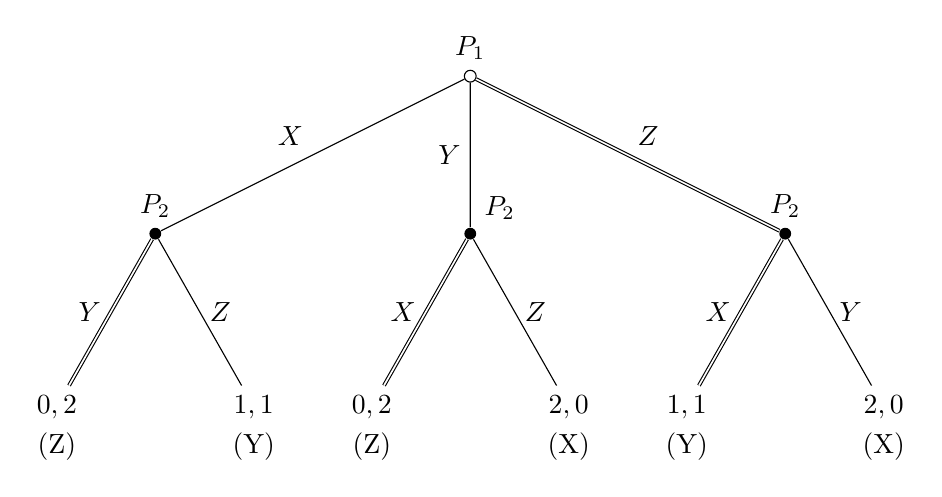
\begin{tikzpicture}[thin,
      level 1/.style={level distance=20mm, sibling distance=40mm},
      level 2/.style={level distance=22mm, sibling distance=25mm},
      every circle node/.style={minimum size=1.5mm,inner sep=0mm}]

      \node[circle,draw,label=above:$P_{1}$] (root) {}
        child { node [circle,fill,label=above:$P_{2}$] {}
          child { 
            node {$0,2$}[double]
			node[below=0.2cm] {(Z)}
            edge from parent
              node[left] {$Y$}}
          child { 
            node {$1,1$}
			node[below=0.2cm] {(Y)}
            edge from parent
              node[right] {$Z$}}
          edge from parent
            node[above left] {$X$}}
        child { node [circle,fill,label=above right:$P_{2}$] {}
          child { 
            node {$0,2$}[double]
			node[below=0.2cm] {(Z)}
            edge from parent
              node[left] {$X$}}
          child { 
            node {$2,0$}
			node[below=0.2cm] {(X)}
            edge from parent
              node[right] {$Z$}}
          edge from parent
            node[left] {$Y$}}
        child { node [circle,fill,label=above:$P_{2}$] {}
          child { 
            node {$1,1$}[double] 
			node[below=0.2cm] {(Y)}
              edge from parent
                node[left] {$X$}}
          child { 
            node {$2,0$}
			node[below=0.2cm] {(X)}
              edge from parent
                node[right] {$Y$}}
           edge from parent
             node[above right] {$Z$}[double]};
    \end{tikzpicture}
	\\\vspace{1em} 
	\scriptsize{Based on exercise 163.2 of Osborne's book: \\ Osborne, Martin J. 2004. \emph{An Introduction to Game Theory.} Oxford: Oxford University Press.}
  \end{figure}

\vspace{4em} % vertical space

%%%%%%%%%%%%%%%%%%%%%%%%%%%%%%%%%%%%%%%%%%%%%%%%%%%%%%%%%%%%%%%%%%%%%%%%%%%%%%%%%%%%%%%%%%%
%
% Extensive form game with imperfect information (highlighting a subgame in red)
%
%%%%%%%%%%%%%%%%%%%%%%%%%%%%%%%%%%%%%%%%%%%%%%%%%%%%%%%%%%%%%%%%%%%%%%%%%%%%%%%%%%%%%%%%%%%

	% Node styles
	\tikzset{
	% Two node styles for game trees: solid and hollow
	solid node/.style={circle,draw,inner sep=1.5,fill=black},
	hollow node/.style={circle,draw,inner sep=1.5}
	}

\begin{figure}[htbp]
	\centering
		\caption{Extensive-Form Game with Imperfect Information (Highlighting a Subgame)}
	\begin{tikzpicture}[scale=1.5,font=\footnotesize]
	% Specify spacing for each level of the tree
	\tikzstyle{level 1}=[level distance=15mm,sibling distance=40mm]
	\tikzstyle{level 2}=[level distance=15mm,sibling distance=22mm]
	\tikzstyle{level 3}=[level distance=15mm,sibling distance=15mm]
	% The Tree
	\node(0)[hollow node,label=above:{$Nature$}]{}
	child{node(1)[solid node]{}
		child{node[label=below:{$(\sigma -1,\gamma - 2)$}]{} edge from parent node[left]{$C$}}
		child{node(3)[solid node,label=right:{$P2$}]{} 
			child{node(4)[label=below:{$(0,0)$}]{} edge from parent node[left]{$E$}}
			child{node(5)[label=below:{$(-10,-10)$}]{} edge from parent node[right]{$F$}}
			edge from parent node[right]{$D$}}
		edge from parent node[right, xshift=3]{$(p)$}	
		edge from parent node[left,xshift=-3]{$A$}
	}
	child{node(2)[solid node]{}
		child{node[label=below:{$(\rho + 1,\tau + 2)$}]{} edge from parent node[left]{$C$}}
		child{node(6)[solid node,label=right:{$P2$}]{} 
			child{node(7)[label=below:{$(0,0)$}]{} edge from parent node[left]{$E$}}
			child{node(8)[label=below:{$(10,10)$}]{} edge from parent node[right]{$F$}}
		edge from parent node[right]{$D$}}
		edge from parent node[left, xshift=-3]{$(p - 1)$}	
		edge from parent node[right,xshift=3]{$B$}
	};
	% information set (from node 1 to node 2)
	\draw[dashed,rounded corners=10]($(1) + (-.2,.25)$)rectangle($(2) +(.2,-.25)$);
	% Highlighting a subgame in red (from node 7 to 8). Remove the code below if you don't want to highlight the subgame.
	\draw[dotted, thick, red, rounded corners=15]($(7) + (-.4,1.75)$)rectangle($(8) +(.4,-.5)$);
	% specify mover at 2nd information set
	\node at ($(1)!.5!(2)$) {$P1$};
	\end{tikzpicture}
\end{figure}



%%%%%%%%%%%%%%%%%%%%%%%%%%%%%%%%%%%%%%%%%%%%%%%%%%%%%%%%%%%%%%%%%%%%%%%%%%%%%%%%%%%%%%%%
%
% Extensive form game with imperfect information and a large information set
%
%%%%%%%%%%%%%%%%%%%%%%%%%%%%%%%%%%%%%%%%%%%%%%%%%%%%%%%%%%%%%%%%%%%%%%%%%%%%%%%%%%%%%%%%

\begin{figure}[htbp]
	\centering
	\caption{Extensive-Form Game with Imperfect Information and a Large Information Set}
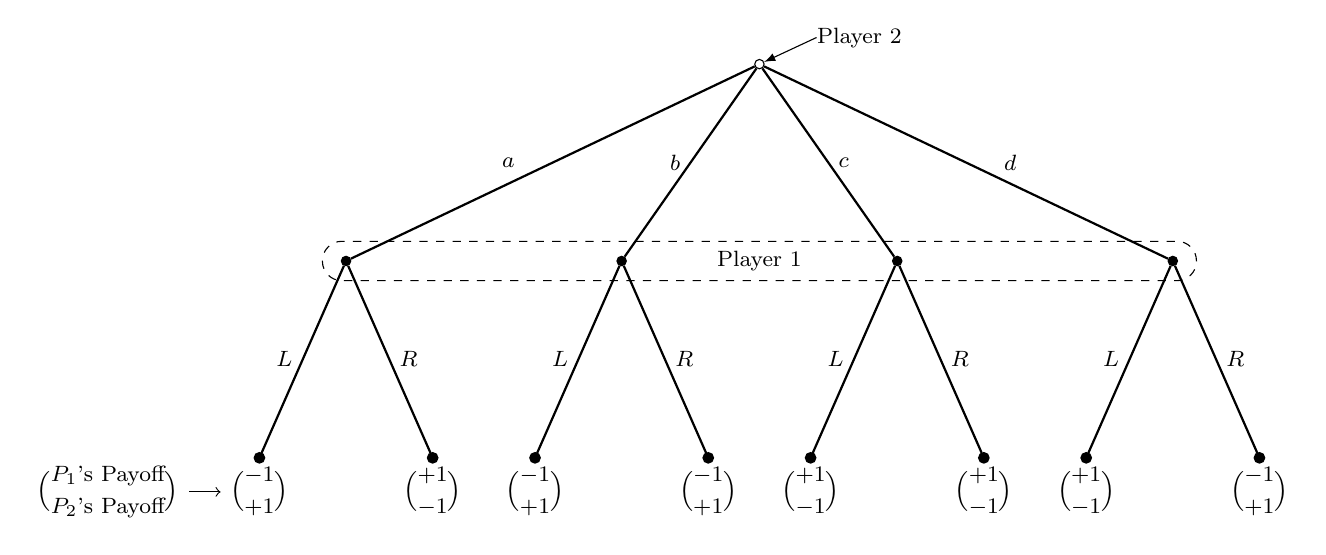
\begin{tikzpicture}[font=\footnotesize,edge from parent/.style={draw,thick}]
  % Two node styles: solid and hollow
    \tikzstyle{solid node}=[circle,draw,inner sep=1.2,fill=black];
    \tikzstyle{hollow node}=[circle,draw,inner sep=1.2];
  % Specify spacing for each level of the tree
    \tikzstyle{level 1}=[level distance=25mm,sibling distance=35mm]
    \tikzstyle{level 2}=[level distance=25mm,sibling distance=22mm]
  % The Tree
  \node(0)[hollow node]{}
    child{node[solid node]{}
      child{node[solid node]{}edge from parent node[left]{$L$}}
      child{node[solid node]{}edge from parent node[right]{$R$}}
      edge from parent node[left,xshift=-10]{$a$}
    }
    child{node[solid node]{}
      child{node[solid node]{}edge from parent node[left]{$L$}}
      child{node[solid node]{}edge from parent node[right]{$R$}}
      edge from parent node[left,xshift=0]{$b$}
    }
    child{node[solid node]{}
      child{node[solid node]{}edge from parent node[left]{$L$}}
      child{node[solid node]{}edge from parent node[right]{$R$}}
      edge from parent node[right,xshift=0]{$c$}
    }
    child{node[solid node]{}
      child{node[solid node]{}edge from parent node[left]{$L$}}
      child{node[solid node]{}edge from parent node[right]{$R$}}
      edge from parent node[right,xshift=10]{$d$}
	    };
	    % information set
	    \draw[dashed, rounded corners=7]($(0-1)+(-.3,.25)$)rectangle($(0-4)+(.3,-.25)$);
	    % specifying movers
	    \draw[<-,>=latex](0)--(25:8mm)node[inner sep=0,right]{Player 2};
	    \node at($.5*(0-1)+.5*(0-4)$){Player 1};
	    % specifying payoffs
	    \node(payoff)[below]at(0-1-1){$\displaystyle\binom{-1}{+1}$};
	    \node[below]at(0-1-2){$\displaystyle\binom{+1}{-1}$};
	    \node[below]at(0-2-1){$\displaystyle\binom{-1}{+1}$};
	    \node[below]at(0-2-2){$\displaystyle\binom{-1}{+1}$};
	    \node[below]at(0-3-1){$\displaystyle\binom{+1}{-1}$};
	    \node[below]at(0-3-2){$\displaystyle\binom{+1}{-1}$};
	    \node[below]at(0-4-1){$\displaystyle\binom{+1}{-1}$};
	    \node[below]at(0-4-2){$\displaystyle\binom{-1}{+1}$};
	    \draw[<-](payoff)--+(-.9,0)node[left]
	      {$\displaystyle\binom{\text{$P_{1}$'s Payoff}}{\text{$P_{2}$'s Payoff}}$};
	  \end{tikzpicture}
	  \\ \vspace{1em} % vertical space
	  \scriptsize{Note: This is Figure 7.D.2 in Mas-Colell, Whinston, and Green's book on microeconomic theory (1995), as replicated by Haiyun Chen (Simon Fraser University).}
	  \end{figure}



%%%%%%%%%%%%%%%%%%%%%%%%%%%%%%%%%%%%%%%%%%%%%%%%%%%%%%%%%%
%
% Game Tree with Curved Information Set
%
%%%%%%%%%%%%%%%%%%%%%%%%%%%%%%%%%%%%%%%%%%%%%%%%%%%%%%%%%%

\begin{figure}[htbp]
	\centering
	\caption{Game Tree with Curved Information Set}\label{curved}
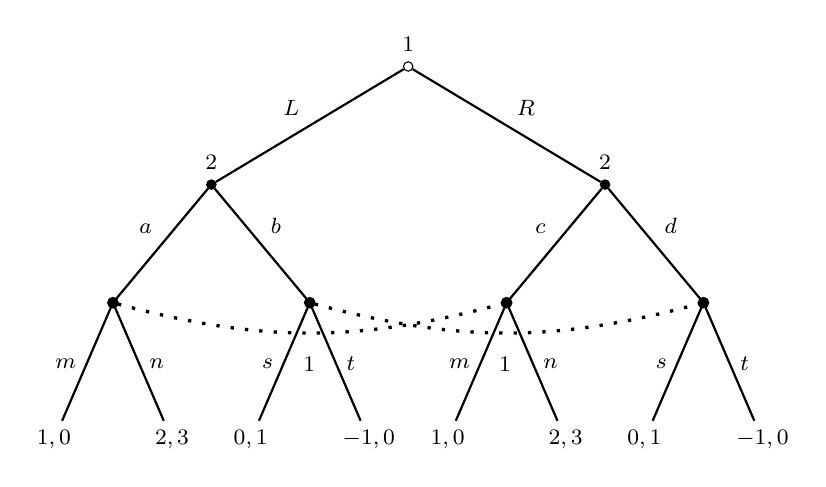
\begin{tikzpicture}[font=\footnotesize,edge from parent/.style={draw,thick}]
  % Two node styles: solid and hollow
    \tikzstyle{solid node}=[circle,draw,inner sep=1.2,fill=black];
    \tikzstyle{hollow node}=[circle,draw,inner sep=1.2];
  % Specify spacing for each level of the tree
    \tikzstyle{level 1}=[level distance=15mm,sibling distance=50mm]
    \tikzstyle{level 2}=[level distance=15mm,sibling distance=25mm]
    \tikzstyle{level 3}=[level distance=15mm,sibling distance=15mm]
  % The Tree
  \node(0)[hollow node]{}
    child{node[solid node]{}
      child{node[solid node]{}
        child{node[below]{$1,0$} edge from parent node[left]{$m$}}
        child{node[below]{$2,3$} edge from parent node[right]{$n$}}
        edge from parent node[above left]{$a$}
      }
      child{node[solid node]{}
        child{node[below]{$0,1$} edge from parent node(s)[left]{$s$}}
        child{node[below]{$-1,0$} edge from parent node(t)[right]{$t$}}
        edge from parent node[above right]{$b$}
}
      edge from parent node[above left]{$L$}
    }
    child{node[solid node]{}
      child{node[solid node]{}
	  child{node[below]{$1,0$} edge from parent node(m)[left]{$m$}}
	          child{node[below]{$2,3$} edge from parent node(n)[right]{$n$}}
	          edge from parent node[above left]{$c$}
	        }
	        child{node[solid node]{}
	          child{node[below]{$0,1$} edge from parent node[left]{$s$}}
	          child{node[below]{$-1,0$} edge from parent node[right]{$t$}}
	          edge from parent node[above right]{$d$}
	  }
	        edge from parent node[above right]{$R$}
	      };
	    % information sets
	    \draw[loosely dotted,very thick](0-1-1)to[out=-15,in=195](0-2-1);
	    \draw[loosely dotted,very thick](0-1-2)to[out=-15,in=195](0-2-2);
	    % movers
	    \node[above,yshift=2]at(0){1};
	    \foreach \x in {1,2} \node[above,yshift=2]at(0-\x){2};
	    \node at($.5*(s)+.5*(t)$){1};
	    \node at($.5*(m)+.5*(n)$){1};
	  \end{tikzpicture}
	   \\ \vspace{1em} % vertical space
	   \scriptsize{Note: This is Figure 6 in Osborne's ``Manual for egameps.sty.''}
	  \end{figure}





%%%%%%%%%%%%%%%%%%%%%%%%%%%%%%%%%%%%%%%%%%%%%%%%%%%%%%%%%%



\end{document}